\cotefile{29}
\scanpage{2}
\uline{Tame ramification}
% archive sheet number: 1
\scanpage{18}
\diagram{\begin{tikzcd}[ampersand replacement=\&,row sep=large]
{{G}'} \arrow[r,-] \& G \\
M' \arrow[r,Rightarrow] \& M
\end{tikzcd}}
% archive sheet number: 17
\scanpage{27}
continu

\[
f^\bullet:\underline{\mathrm{Et}}_S\qquad\underline{\mathrm{Et}}_T\quad .
\]

On suppose donné une donnée de ramification $\underline{R}_S=(\underline{C}_S,\underline{s}_S)$ sur $S$, une autre $\underline{R}_T=(\underline{C}_T,\underline{s}_T)$ sur $T$, et un foncteur \inserted{noté} $M\quad M\mathbin{\mathrm{x}}_S T:\underline{C}_{\unsure{S|T}}\quad\underline{C}_T$, transformant morphismes cartésiens en morphismes carétsiens et rendant commutatif de diagramme

\diagram{\begin{tikzcd}[ampersand replacement=\&,column sep=large]
\underline{C}_S \& \& \underline{C}_T\\
\underline{\mathrm{Et}}_S \& {f^\bullet} \& \underline{\mathrm{Et}}_T\quad .
\end{tikzcd}}

Considérons de plus le carré de foncteurs

\diagram{\begin{tikzcd}[ampersand replacement=\&,column sep=small,row sep=small]
\underline{C}_S \& \& \underline{C}_T\\
\underline{s}_S \& \& \underline{s}_T\\
(\mathrm{Sch})_{/S} \& \& (\mathrm{Sch})_{/T}\\
\& {X\quad X\mathbin{\mathrm{x}}_S T} \&
\end{tikzcd}}

et supposons donné un morphisme $u$ entre les deux composés:

\[
u(M):\quad\underline{s}_T(M\mathbin{\mathrm{x}}_S T)\qquad
\underline{s}_{\deleted{\unsure{T}}S}(M)\mathbin{\mathrm{x}}_S T
\]

qui, pour tout $M$ fixé\deleted{\unsure{, soit un}} sur $S'\quad\mathrm{Ob}\,\underline{\mathrm{Et}}_S$, soit un ${\unsure{F|f}}^{\bullet}(S')$-morphisme. Sous ces conditions, on définit de façon évidente un foncteur, noté $f^\bullet$ \inserted{ou $M\quad M\mathbin{\mathrm{x}}_S T$} si une confusion n'est pas à craindre, de $\mathrm{Rev}^{\underline R}(S)$ dans $\mathrm{Rev}^{\underline R_T}(T)$ et un homomorphisme de foncteurs composés

\diagram{\begin{tikzcd}[ampersand replacement=\&,column sep=small]
\mathrm{Rev}^{\underline R(S)}(S) \& \& \mathrm{Rev}^{\underline R(T)}(T)\\
\mathrm{Rev}(S) \& \& \mathrm{Rev}(T)\quad .\\[-1ex]
\& {X\quad X\mathbin{\mathrm{x}}_S T} \&
\end{tikzcd}}

Cet homomorphisme est un isomorphisme dans certains cas, par exemple sous les conditions de l'exemple 3, lorsqu'on suppose (sous les notations d'icelui) que pour tout sous-groupe $H$ de $G$, le passage au quotient $\underline{s}(M)/H$ commute au changement de base $T\quad S$; cette condition sera vérifié
% archive sheet number: 26
\scanpage{28}
par exemple si $T\quad S$ est\unsure{h} plat, ou dans le\deleted{s cas} kummérien\deleted{s} \inserted{a)} envisagé\deleted{s} plus haut (en supposant que les images inverses des $D_i$ dans $T$ existent, et prenant ces derniers pour définir une donnée de recollement sur $T$).

On recule devant la tâche d'expliciter une propriété de transitivi- pour un composé $U\quad T\quad S$, et jetant provisoirement un voile pudique sur ces abimes, nous allons remarquer plûtôt que le foncteur $\mathrm{Rev}^{\underline R(S)}(S)\qquad\mathrm{Rev}^{\underline R(T)}(T)$ qu'on vient de construire a le bon goût d'être \uline{exact}. Si alors , dans les conditions de l'exemple 3, $\quad$ est un point géométrique de $T$, \deleted{non ramifié pour les données $\underline R_{(\unsure{T})}$}\inserted{non ramifié pour $\underline R(T)$,} dont l'imgge dans $S$ est non ramifié pour $\underline R_{(S)}$, et si on suppose que \deleted{$\underline R_{(T)}$ est l'image inverse de $\underline R_{(S)}$, alors} l'homomorphisme \inserted{$u$ dans} $(\unsure{*|=})$ de foncteurs composés induit un isomorphisme sur les fibres géométriques en $\quad$, alors les sorites de Exp V impliquent qu'on a un homomorphisme canonique $ {}_{1}^{\underline R(\deleted{S}\unsure{T|S})}(\deleted{S}T,{}_{\deleted{S}T})\qquad{}_{1}^{\underline R(S)}(S,{}_{S})$. Ceci s'applique en particulier au cas de données kummériennes type a), ou type b) \inserted{$1^{\underline{\mathrm o}}$ et $2^{\underline{\mathrm o}}$;} quand on suppose que $T\quad S$ est un morphisme régulier \unsure{resp.|repp.} lisse (de sorte que l\deleted{es}'image\deleted{s} inverse\deleted{s} de\deleted{s} $D_{\deleted{i}}$ satisf\unsure{a}it encore aux mêmes conditions de ``normal crossings'' que $D$ lui-même).

Il y a a expliciter deux cas particuliers importants de fonctorialité. L'un est celui où $T\quad S$ est étale, et où $\underline R_{(T)}$ est induit par $\underline R_{(S)}$ sur $S$, auquel le \deleted{foncteur} carré nous était déjà connu par ailleurs (et l'homomorphisme de foncteurs composés y est un isomorphisme), puisque l'on dispose d'un foncteur cartésien $\underline{\mathrm{Rev}}^{R}\qquad\underline{\mathrm{Rev}}$ sur $\underline{\mathrm{Et}}_S$. Lorsqu'on suppose de plus $T$ fini sur $S$, $S$ et $T$ connexes, et qu'on est dans les conditions de l'exemple 3, alors l'homomorphisme sur les groupes \unsure{fondamentau|fondamentaux} est un monomorphisme, dont l'image est le sous-groupe de $ {}_{1}^{\underline R}(S,\quad)$ défini par le revêtement ponctué $T$ de $S$. Le deuxième cas est celui \unsure{où} $T\quad S$ est \unsure{un} \unsure{morphisme} entier, radiciel et surjectif, et où $\underline R_{(T)}$
% archive sheet number: 27
\scanpage{30}
de se borner aux données de ramification $\underline R$ du type envisagé dans l'exemple 3; ce sont les seules sans doute qu'on rencontrera jamais, et les seules aussi où on sait construire le foncteur réalisation géométrique $\underline r$ et en dire des choses raisonnables.

Avec l'une ou l'autre approche mentionnée à l'alinéa précédent pour traiter de données de ramifications sur des schémas variables sur $S$, (et toujours sous les conditions de l'exemple 3 ...) on est en condition pour énoncer et démontrer qu\deleted{e}'un morphisme fidèlement plat et quasi-compact $T\quad S$ est de descente effective pour la catégorie fibrée sur $(S,T,T\mathbin{\mathrm{x}}_S T,T\mathbin{\mathrm{x}}_S T\mathbin{\mathrm{x}}_S T)$ formée des revêtements de type $\underline R_{(S)}$ ,..... Ceci s'appliquera en particulier à la \unsure{descente|desente} fidèlement plate des revêtements kummériens; c'est utilisé (sans démonstration) à la page 38 des notes de Murre dans le cas de la \unsure{desente|descente} à partir d'un anneau complété, sans compter diverses utilisations de descente à partir d'un localisé strict. Il y a également lieu d'énoncer une propriété de passage à la limite, pour un système projectif $(\unsure{S|X}_i)$ de schémas quasi-compacts et quasi-séparés à morphismes de transition affines; cela permettra de ramener ce qui se passe au voisinage d'un point $s$ d'un $S$ à voir ce qui se passe en $\mathrm{Spec}(\underline O_{S,s})$. Par exemple, dans le cas $S$ \inserted{loc noeth} normal munie d'une famille $(D_i)_{i\;\;I}$ de diviseurs réduits, donc où \inserted{la catégorie} des revêtements kummériens s'identifie\deleted{nt} à \deleted{\unsure{des}} une sous-catégorie de la catégorie des revêtements, on trouve que le revêtement $X$ de $S$ est \deleted{\unsure{norm}} kummérien sss pour tout $s\quad S$, il en est de même du revêtement induit sur $\mathrm{Spec}(\underline O_{S,s})$, et on peut dans cet énoncé remplacer $\underline O_{S,s}$ son hensélisé ou par son hensélisé strict, \deleted{Il y aura un énoncé \unsure{a}} voire par son complété si les hypothèses faites restent stables
% archive sheet number: 29
\scanpage{34}
e) Etant donnés deux objets $M,M'$ de $\underline C_{S'}$, il existe une famille couvrante de morphismes $S'_i\quad S'$ dans $\underline{\mathrm{Et}}_S$, telle que pour tout $i$, \deleted{\unsure{L|M}}les images $M_i$ et $M'_i$ de $M$ et $M'$ sur $S'_i$ soient dominés par un même objet $M''_i$ de \deleted{Ob} $\underline C_{S'_i}$.

Lorsqu'on adopte cette présentation, on peut, dans la des\unsure{c|e}ription des données de ramification kummériennes, se dispenser d'introduire aussi des isomorphismes \deleted{\unsure{G|a}} $u:G_{S'}\qquad{}_{n\;S'}$.
% archive sheet number: 33
\scanpage{40}
\uline{\unsure{Finitudes|Finitude}}

(Pbs et conjectures)
% archive sheet number: 39
\scanpage{41}
Théorèmes de finitude pour le groupe fondamental

1) Sur un corps \unsure{séparablement|algébriquement} clos:

\[
\text{a)}\qquad X\ \text{propre}\,/k\quad\Longrightarrow\quad\pi_1(X)\ \text{de type fini}
\]

\diagram{\begin{tikzcd}[ampersand replacement=\&,column sep=small,row sep=large,execute at end picture={\draw[gray] (pb.north) .. controls ([xshift=10mm]pb.north east) and ([xshift=8mm]pc.south east) .. (pc.south) .. controls ([xshift=-8mm]pc.south west) and ([xshift=-8mm]pb.north west) .. (pb.north);}]
{\text{b)}\quad X\ \text{t.f.}\,/k} \& \Longrightarrow \& |[alias=pb]| {\pi'_1(X)} \& {\text{de }\boxed{\text{\uline{présentation}}}\ \text{\uuline{finie}}}\\
{\text{c)}\quad X\ \text{t.f.}\,/k} \& \Longrightarrow \& |[alias=pc]| {\pi_1^t(X)} \arrow[u] \& {\text{de type fini}}
\end{tikzcd}}

\margin{($'$ indique partie première à la caractéristique)}

\margin{($t$ indique que la ramification est tame sur \unsure{tt|H} \deleted{\unsure{modèle} propre} \inserted{``diviseur''} \deleted{d'une \unsure{comp.|corps}} du corps de fonctions des composantes irréd]}

[N.B. c) plus général que a)]

\margin{$X_i\subset X$ irréd. \unsure{composantes|composant}}

a) \uline{démontré}, [par \uline{descente} réduction au cas normal, par \uline{Bertini} au cas d'une courbe, puis théorie de spéc. du gpe fond. et méthode \unsure{transcendante|transcendance}]

\deleted{b) \inserted{\unsure{le type fini est prouvé}} [réduit au cas $X$ normal [descente] \unsure{par}]}

b) Le cas ``\uline{type fini}'' est \unsure{prouvé|présumé} [réduction au cas normal par descente puis au cas non singulier ``joli'' du sens Artin, on utilise alors la suite exacte des $\pi_1$ i.e. th. de spécialisation du \unsure{grpe.|gpe} fond, qui nous ramène au cas d'une courbe normale, où on est ramené par th. de spéc. au cas \unsure{transcendant}]

\unsure{Enfin|A priori|Espoir|Quid} : \unsure{ceci}, on est ramené pour b) au cas $X$ \uline{normal} [descente] et \unsure{même} [via \uuline{résolutions}] au cas $X$ \deleted{\uline{régulier}}\inserted{lisse/$k$}. \uline{Si} $X$ \deleted{\unsure{projectif|propre}]}\unsure{est|on est} [\uline{Lefschetz}] ramené, au cas d'une surface. Si on a \unsure{résolution} sous forme forte, \uline{cas} d'une surface \unsure{projective}, \deleted{intersection} \deleted{\unsure{complète|complété}}\inserted{lisse} diviseur (à normal crossings).

\deleted{c)}
% archive sheet number: 40
\scanpage{42}
\figure{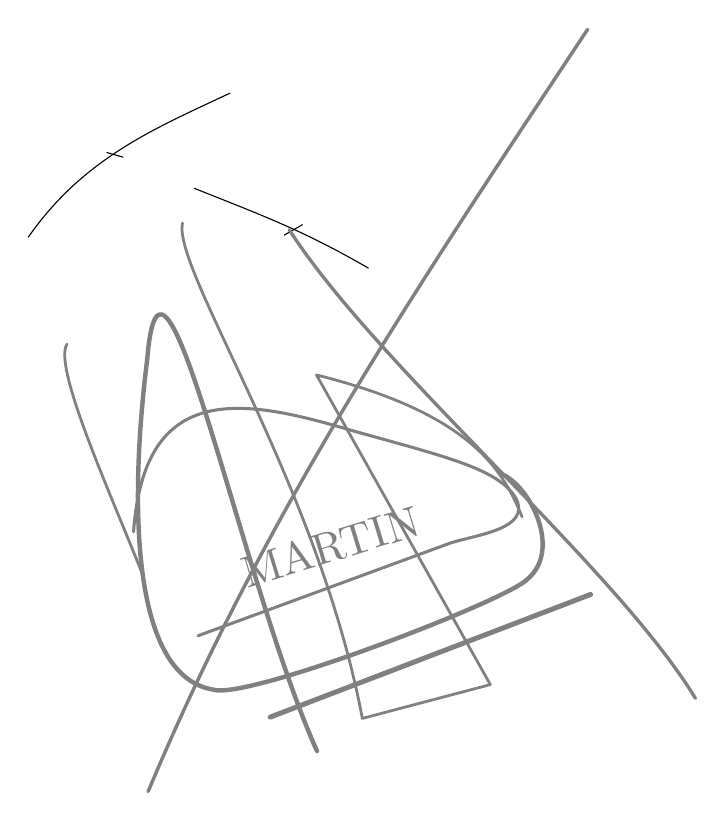
\begin{tikzpicture}[x=.64cm,y=-.53cm,line cap=round,line join=round]
\draw (1.8,6) .. controls (2.9,4.1) and (4.3,3.4) .. (5.8,2.55);
\draw (3.36,3.97)--(3.68,4.08);
\draw (5.1,4.83).. controls (6.6,5.55) and (7.3,5.87)..(8.55,6.74);
\draw (6.88,5.95)--(7.24,5.7);
\draw[gray,line width=1.25pt] (12.9,1.02).. controls (9.4,7.4) and (6.5,12.6)..(4.18,19.28);
\draw[gray,line width=1pt] (4.86,5.66).. controls (4.67,6.8) and (7.55,11.9)..(8.43,17.53)--(10.97,16.72)--(7.52,9.3).. controls (10.5,10.2) and (11.2,11.5)..(11.6,12.7);
\draw[gray,line width=1.2pt] (6.98,5.82).. controls (8.72,9.1) and (13.46,13.9)..(15.04,17.05);
\draw[gray,line width=1.6pt] (7.53,18.31) .. controls (6.03,14.3) and (4.45,4.6) .. (4.16,8.94) .. controls (3.85,11.9) and (3.74,16.5) .. (5.47,16.84) .. controls (6.13,17.1) and (11.27,14.72) .. (11.7,14.2) .. controls (12.4,13.5) and (11.77,11.95) .. (11.17,11.66);
\draw[gray,line width=1pt] (2.57,8.56).. controls (2.27,9.1) and (3.52,12.37)..(4.08,14.12);
\draw[gray,line width=1.1pt] (3.89,13.06).. controls (4.1,9.49) and (5.98,9.83)..(8.16,10.61).. controls (10.04,11.25) and (11.14,11.54)..(11.48,12.26).. controls (11.78,12.99) and (10.72,13.12)..(10.17,13.33)--(5.17,15.55);
\draw[gray,line width=1.8pt] (6.6,17.5)--(12.96,14.56);
\node[rotate=17,scale=1.6,text=gray] at (7.8,13.42){\unsure{MARTIN}};
\end{tikzpicture}}
% crop-candidate: scan 42

\deleted{$A$ anneau noethérien}

\deleted{$x,y\in A$}

\deleted{a) $A/x$, \inserted{$A/y$} réguliers \inserted{intègres} de dim $1$}

\deleted{b) $A$ \inserted{séparé et} complet pour la topologie définie par $xy$}

\diagram{\begin{tikzcd}[ampersand replacement=\&]
\widehat A^{(x)} \& \& {\deleted{\widehat A^{(y)}}}\\
\& A \arrow[ul]\arrow[ur] \&
\end{tikzcd}}

\diagram{\begin{tikzcd}[ampersand replacement=\&]
\widehat X^x \arrow[dr] \& \& {\deleted{\widehat X^y}} \arrow[dl]\\
\& {\deleted{X}} \&
\end{tikzcd}}

\[
\widehat A^{(x,y)}=k[[x,y]]
\]

\figure{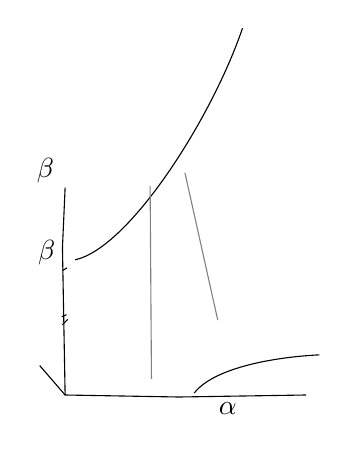
\begin{tikzpicture}[x=.85cm,y=.85cm]
\draw (0,3.1)--(-.04,2.2)--(0,0)--(1.7,-.03)--(3.6,0);
\draw (-.04,1.05)--(.04,1.13) (-.05,1.17)--(.02,1.2) (-.04,1.86)--(.03,1.9);
\node[left] at (-.02,3.35){$\beta$}; \node[left] at (0,2.13){$\beta$}; \node[below] at (2.43,.04){$\alpha$};
\draw (.15,2.02)..controls (.96,2.2) and (2.19,4.13)..(2.65,5.48);
\draw (1.93,.03)..controls (2.2,.38) and (3.02,.56)..(3.8,.6);
\draw[gray,thin] (1.27,3.12)--(1.29,.24) (1.79,3.32)--(2.28,1.12);
\draw (-.38,.44)--(0,0);
\end{tikzpicture}}

\[
\begin{aligned}
\widehat A^{x}&=\left\{\sum a_{\alpha\beta}\,x^{\unsure{\alpha|\gamma}}y^\beta\right\}\\
&\text{\unsure{seul|dont} un nb fini de termes, pour $\alpha\leq N$ donné, sont non nuls}\\
&=k[y][[x]]
\end{aligned}
\]

\[
\begin{aligned}
\widehat A^y&=\left\{\sum a_{\alpha\beta}\,x^\alpha y^\beta\right\}\\
&\text{\unsure{seul|dont} \uline{un} nb fini de termes pour $\beta\leq N$ donné sont non nuls}\\
&=k[x][[y]]
\end{aligned}
\]

\[
\begin{aligned}
&\deleted{\unsure{\beta=}}\\
A&=\left\{\sum a_{\alpha\beta}\,x^\alpha y^\beta\right\}\\
&\text{seul un nb fini des $a_{\alpha\beta}$ pour $\alpha+\beta\leq{}$\uline{$N$ donné}, sont non nuls}
\end{aligned}
\]
% archive sheet number: 41
\scanpage{43}
c) \inserted{\uline{Prouvé}} Modulo \uline{conjecture} d'\unsure{invariance} \unsure{birationnelle|birat. abs|birat. rel} de la ramification modérée \inserted{[si $X$ non \deleted{\unsure{pro}} projective]} [qui donne un sens au pb.] et procédant comme dans b) [\deleted{Lefschetz, résolution}\inserted{\unsure{normalisation}, Bertini...}] on est ramené à une \deleted{surface \unsure{projective}}\inserted{\uline{courbe}} lisse, -- OK.

\deleted{\unsure{et} diviseur à croisements normaux, OK.}

2) \uline{Groupe fondamental local}.

$X$ \deleted{\unsure{spectre}} schéma noeth. $\left\{\begin{array}{l}\text{\unsure{complet|complète}}\\\text{\uline{str.} \uline{local} et \uline{bon}.}\end{array}\right.$

$U$ un ouvert. A prouver

a) $\pi_1^t(U)$ de type fini

b) $\pi'_1(U)$ de présentation finie

Via résolution, et conjecture de \unsure{tameness|fameuse} (\unsure{invariance} \unsure{birationnelle|birationelle}) dans le cas a), on doit s'en tirer, en se réduisant aux énoncés analogues \deleted{\unsure{pour}} de 1)......

a) Par descente, on est ramené au cas $X$ normal, et par Lefschetz [du moins \uline{si $U=X-\text{origine}$}] au cas où $\dim X=2$. On dispose alors de Abhyankar, et cela doit marcher.....

% slanted
\margin{vérifier si c'est \uline{nécessaire}}
% archive sheet number: 42
\scanpage{44}
\deleted{$\mathfrak X$ \inserted{\unsure{pré}}schéma formel loc. noeth.}

\deleted{$\mathfrak X_0$ un sous-schéma de définition, $X_0=\mathrm V(\unsure{\mathcal J|\mathcal I})$}

\deleted{On \unsure{a|va} définit la catégorie $\mathrm{Coh}(\mathfrak X/\mathfrak X_0)$ des ``\deleted{revêtements finis}\inserted{Modules \unsure{Cohérents|cohérents}} de $\mathfrak X$ mod $X_0$''\unsure{\}}. Soit $\mathrm{Coh}(\mathfrak X)$ la catégorie des \deleted{schémas formels finis}\inserted{modules Coh.} sur $\mathfrak X$. \deleted{Soit} Soit $\unsure{\mathscr F|\mathscr S|\mathfrak S}$ l'ensemble des flèches de $\mathrm{Coh}(\mathfrak X)$ telles que $\mathrm{Ker}\,u$ et $\mathrm{Coker}\,u$ soit \deleted{\unsure{p. à p. par}} annulé \deleted{par}\inserted{loc.} par une puissance de $\mathcal J$. Alors l'ens. $\mathscr F$ \deleted{\unsure{est}} satisfait aux axiomes qu'il faut pour passer à une catégorie de fractions [N.B. on pense en particulier \unsure{évid.} à la sous-catégorie épaisse des Modules coh. tués par \unsure{un|une} $\unsure{\mathcal J^n|\mathcal J}$].}

\deleted{$\mathrm{Coh}(\mathfrak X/\mathfrak X_0)$ est la catégorie des fractions.}

\deleted{\uline{Exemple} Soit $X$ propre sur $Y=\mathrm{Spec}\,A$, $A$ noeth séparé et complet pour idéal $I$, $Y_0=\mathrm V(I)$, $X_0=X\times_Y Y_0$, $\mathfrak X$ le complété formel de $X$.}

\deleted{Alors}

\diagram{\begin{tikzcd}[ampersand replacement=\&,row sep=large]
\deleted{\mathrm{Coh}(\mathfrak X)} \& \deleted{\mathrm{Coh}(X)} \arrow[l,"\simeq"'] \& {\text{\deleted{par le th. d'existence}}}\\
\deleted{\mathrm{Coh}(\mathfrak X)_{\text{\unsure{négl|nilp}}}} \arrow[u,hook] \& \substack{\deleted{\mathrm{Coh}(X)_{\text{négl}}}\\\text{\deleted{(support $\subset X_0$}}} \arrow[u,hook] \&
\end{tikzcd}}

On trouve $\mathrm{Coh}(\mathfrak X/\mathfrak X_0)\cong\mathrm{Coh}(X-X_0)$ !
% archive sheet number: 43
\scanpage{45}
3) \uline{Théorèmes de finitude simultanés}

\unsure{Concernant|Concernent|Comment} les groupes fondamentaux des fibres \inserted{\unsure{géom.}} d'un morphisme de type fini : on désire des résultats genre constructibilité, \unsure{généralisant} a), b), c):

a) Majoration \deleted{``\unsure{groupe théorétique|gruppen theoretisch|group-theoretical}''}\inserted{uniforme} des nb de générateurs \unsure{des|dans} $\pi_1(X_{\bar s})$, si $X/S$ \uline{propre} O.K.

% slanted
\margin{c'est fait}

b) Majoration \inserted{uniforme} des nb de générateurs et de relations pour les $\pi'_1(X_{\unsure{\bar p|\bar s}})$, ou \uline{mieux}: la structure de $\pi'_1(X_{\bar p})$ est fonction \uline{constructible} de $s$

c) Majoration uniforme des nb de générateurs des $\pi_1^t(X_{\bar s})$.

Il semble que les méthodes qui résoudront \unsure{1)|4)} résoudront également 3).
% archive sheet number: 44
\scanpage{46}
On définit une catégorie $\unsure{R|\mathscr R}(\mathfrak X/\mathfrak X_0)$ ainsi.

$R(\mathfrak X)=$ catégorie des $\mathfrak X$-préschémas formels finis sur $\mathfrak X$.

\deleted{On définit la \unsure{catégor.|catégorie} des flèches $S$ [isom mod $\mathfrak X_0$] par $u:\mathfrak X'\mathbin{-}\mathfrak X''$ est un isom mod $\mathfrak X_0$ sss l'hom d'Algèbres $\mathcal A''\mathbin{-}\mathcal A'$ correspondant est un isom de Modules mod $X_0$. On vérifie qu'on obtient un calcul des fractions à droite [stable par composition, stable par changmt de base, égalisation]. La catégorie quotient est notée $R(\mathfrak X/\mathfrak X_0)$.}

\deleted{\uline{Exemple} Reprenons l'exemple précédent. Alors $R(\mathfrak X)\xleftarrow{\simeq}\unsure{\mathbb R|R}(X)$ par le théorème de comparaison, donc $R(\mathfrak X/\mathfrak X_0)$ est équivalente : $R(X/X_0)$, qu'on vérifie être équivalente à $R(X-X_0)$.}

\deleted{[$R(X/X_0)\mathbin{-}R(X-X_0)$, c'est \uline{\unsure{flt.|plt.|fth.} fidèle} comme on vérifie directement, c'est ess. surjectif comme on voit grâce à la version globale du Main Theorem p.ex. .....] .}

% slanted
\margin{\uline{à vérifier}}
% archive sheet number: 45
\scanpage{47}
Th. de \unsure{finitude|finitudes} \uline{relatif} pour $\pi_1$
% archive sheet number: 46
\scanpage{48}
\mspage{I}

\deleted{\uline{\unsure{Proposition}}}

\uline{Lemme 1} Soit $f:X\mathbin{\text{---}}Y$ un morphisme \deleted{\unsure{propre} surjectif de t.f., à fibres géom. connexes, $Y$ \unsure{localt} noeth.} \inserted{fid. plat \deleted{\unsure{normal}} \unsure{biréduit|réduit} \deleted{plat normal}} \inserted{de préschémas loc. noethériens, avec $Y$} normal intègre pt gén. $y$, et soient $X'$, $X''$ deux rev. étales de $X$, tels que $X'_{\bar y}$ \deleted{\unsure{soit|et}} \inserted{et} $X''_{\bar y}$ soit $X_{\bar y}$-isomorphes. \inserted{On suppose $X_{\bar y}$ connexe.} \deleted{Alors $\exists$ revêtement fini étale $Y'_1$ de $Y$ tel que $X'\times_Y Y_1$ et $X''\times_Y Y_1$} soient $X\times_Y Y_1$-isomorphes.

Plus précisément, \inserted{\unsure{pour|par}} tt hom (isom) $\bar u:X'_{\bar y}\mathbin{\text{---}}X''_{\bar y}$, si $K'_1$ est la \deleted{\unsure{sous}} \inserted{plus petite} extension de $k(\bar y)=\overline{k(y)}$ sur $k(y)$ sur laquelle \unsure{elle|il} est défini, alors \deleted{\unsure{le|si}} $K'_1$ est \uline{étale} sur $Y$, \deleted{et $\bar u$ est défini} \inserted{i.e. le normali\unsure{sé}} $Y_1$ de $Y$ dans $K'$ est étale sur $Y$, et $\bar u$ provient d'un \inserted{$X\times_Y Y_1$-}hom (isom) \inserted{unique} $X'\times_Y Y_1\mathbin{\text{---}} X''\times_Y Y_1$.

Pour le voir, introduisant $\underline{\mathrm{Hom}}_X(X',X'')$ resp. $\underline{\mathrm{Isom}}_X(X',X'')$, on peut supposer que $X'=X$, D'autre part, on peut supposer \unsure{initialemt|initialement|inversement} $Z=X''$ connexe (quitte à le remplacer par la composante connexe de l'image de $X_{\bar y}\xrightarrow{\bar u} Z_{\bar y}\mathbin{\text{---}} Z$). L'hyp. indique que $Z_y$ est de la forme $\deleted{Z}X\times_y y_1$\inserted{ (SGA $\boxed{\mathrm{IX}}$ 6.2.)}, où $y_1$ est une \unsure{ext.|rev.} étale connexe de $y$, qu'on peut supposer contenue dans $\overline{k(y)}$, \deleted{\unsure{pour}} de \uline{façon} que $\bar u$ est défini par l'inclusion $k(y_1)\mathbin{\text{---}}\overline{k(y)}$.
% archive sheet number: 47
